\documentclass{article}

\usepackage{xeCJK}
\setCJKmainfont{SimSun}

\title{FPGA Homework III}
\author{李约瀚 \\ 14130140331 \\ qinka@live.com \\ qinka@qinka.pw}

\usepackage{listings}
\usepackage{hyperref}

\begin{document}
    \maketitle
    \newpage
    \section{Get Started}
    \label{sec:getstarted}
    
    For this homework, the best way to get a funny but valued VHDL project which can run on the Nexys, is search on the GitHub.
    So I seach the key word \verb|Nexys3| and limit the language: \lstinline|language:VHDL|.
    And then I find a repo is about play the game ``snake'' with Nexys3\footnote{\url{https://github.com/kaanege/snake-vhdl}}.
    I forked that repo to my own, and using ISE to do the rest of things.
    
    \subsection{Clone and Create Prj}
    \label{sec:cloneandcreateprj}
    
    The easiest thing to do is clone a repo, just using:
    \begin{lstlisting}
$ git clone git@github.com:Qinka/snake-vhdl.git
    \end{lstlisting}
    And then create an ISE project with the name \verb|FPGA-Snake|, and add the codes via ``coping''.
    
    Before whatever there are, the first thing to do without thinking is ``Synthesize XST''.
    It cost a lot of time to synthesize this example.
    
    \section{Puzzle}
    \label{sec:puzzle}
    
    Now, let we analyze how it does work.
    
    \subsection{Clock Unit}
    \label{sec:clockunit}

    First unit is clock unit, \verb|clock_divider.vhd|. This clock unit has two input pins and two output pins.
    Input pins include a 100MHz clock input port and a reset port, which is used to reset the clock.
    One of output pins can output a 25MHz clock signal, and other output port is a counter-down.
    
    The 100MHz clock is linked to peripheral clock, whose frequency is 100 MHz, too.
    The reset port with it's signal will hold the clock, when reset signal is set up to 1.
    When the reset signal turn over to 0, the clock will output the clock signal in the next cycle's rising edge.
    
    \subsection{VGA Unit}
    \label{sec:vgaunit}
    
    VGA Unit is the part which send the video signals to screen. It has three input ports and seven output ports.
    For input, there are some ports for reset signal, vga clock signal, and a port named \verb|borad_out|,
    which means the context for outputs, including border, space, food,and the tails of the snake.
    At the same times, it will output the vertical synchronous signal and horizontal synchronous signal,
    as same as the signals about red, green, and blue.
    
    For each pixel, there should a clock rising edge(the signal), and the context about the type of this pixel.
    It will send the sync-signal to screen, and at the same times, it will generate the red, green, and blue signals for
    screen to display.
    
    We can change the color of the each kind of item, when not liking them.
     
     \subsection{Game Logic Unit}
     \label{sec:gamelogicunit}

     Game logic unit is about to control game. There are eight input ports and two output ports. 
     The two output are the reset signal when game was overm and the state signal when the state changed.
     % ready,directioncheck,check,move,generatefood,game_over,vga
     The states are included ``ready'', ``directioncheck'', ``check'', ``move'', ``generatefood'', ``game_over'' ,``vga''.

     The input ports include clock signal, reset signal, direction signal, vertical sync-signal, random food, cell, and location. 6 5

    
    \section{Pre-Simulation}
    \label{sec:presimulation}
    
    This example do not provide test bench, so here, I need to write these test benches by myself.
    
    \subsection{Clock Unit}
    \label{sec:ps:clockunit}
    
    To test, simulation and verification this unit, firstly, the test bench file is necessary.
    Then we comment the processes for the \verb|clk25| and \verb|clkdeb|, beacuse these two processes
    try to input a signal to a output register.
    Then we need to create a process for reset signal and a constant var for reset signal period.
    
    Then the final test bench is:
    \begin{lstlisting}[language=VHDL,caption=Clock Unit Test Bench]
LIBRARY ieee;
USE ieee.std_logic_1164.ALL;

ENTITY tb_clock_divider IS
END tb_clock_divider;

ARCHITECTURE behavior OF tb_clock_divider IS 

COMPONENT clock_divider
    PORT(
        clk100 : IN  std_logic;
        reset  : IN  std_logic;
        clk25  : OUT  std_logic;
        clkdeb : OUT  std_logic
    );
END COMPONENT;

-- input
signal clk100 : std_logic := '0';
signal reset  : std_logic := '0';
[language=VHDL,caption=VGA]--output
signal clk25  : std_logic;
signal clkdeb : std_logic;
--constant
constant clk100_period : time := 10  ns;
constant clkdeb_period : time := 10  ns;
constant rst_period_1  : time := 666 ns;
BEGIN

    uut: clock_divider PORT MAP (
        clk100 => clk100,
        reset  => reset,
        clk25  => clk25,
        clkdeb => clkdeb
    );

    clk100_process :process
    begin
        clk100 <= '0';
        wait for clk100_period/2;
        clk100 <= '1';
        wait for clk100_period/2;
    end process;

    rst_process_1 : process
    begin
        reset <= '1';
        wait for 10 ns;
        reset <= '0';
        wait for rst_period_1;
        reset <= '1';
        wait for 100 ns;
        reset <= '0';
        wait for 100 ms;
    end process;

    stim_proc: process
    begin	
        wait for 100 ns;	
        wait for clk100_period*10;
        wait;
    end process;
END;
    \end{lstlisting}
        
    Then we can check behavioral syntax and simulate. Then we will get the output like figure \ref{fig:homework3-1},
    figure \ref{fig:homework3-2}, and figure \ref{fig:homework3-3}.
    
    \begin{figure}[h]
      \centering
      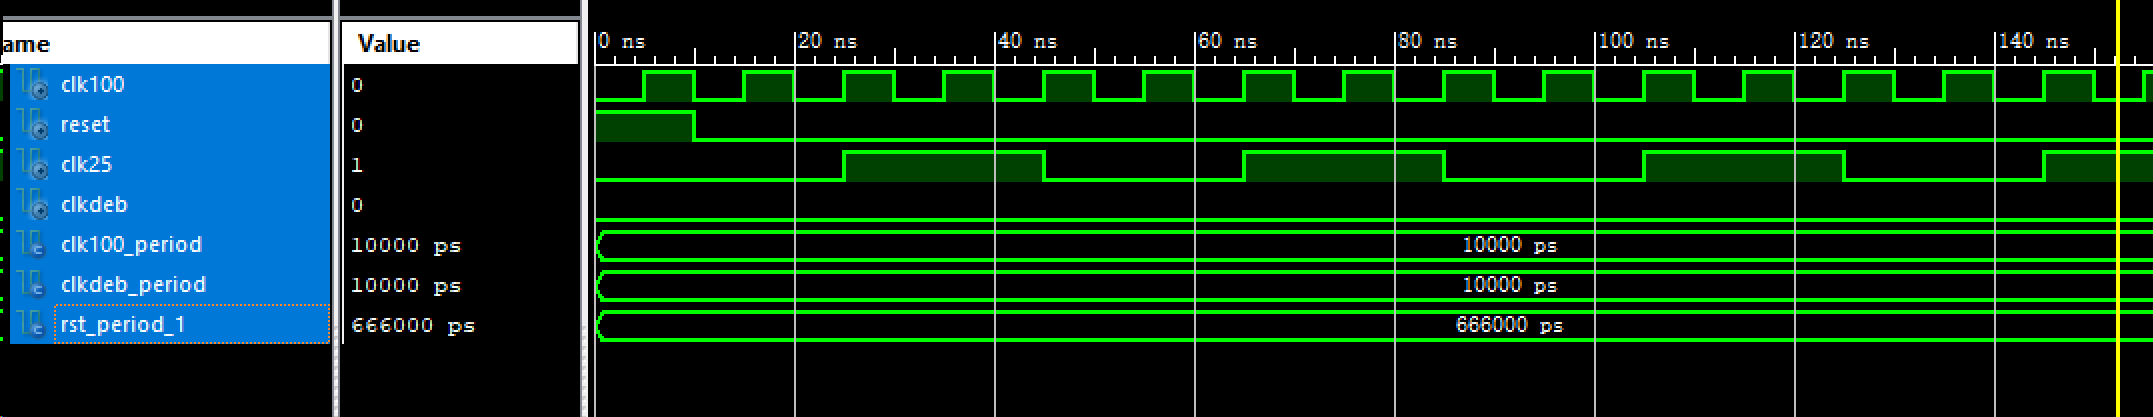
\includegraphics[width=1\linewidth]{homework3-1}
      \caption{The Simulation of Clock Unit (1)}
      \label{fig:homework3-1}
    \end{figure}
    \begin{figure}[h]
      \centering
      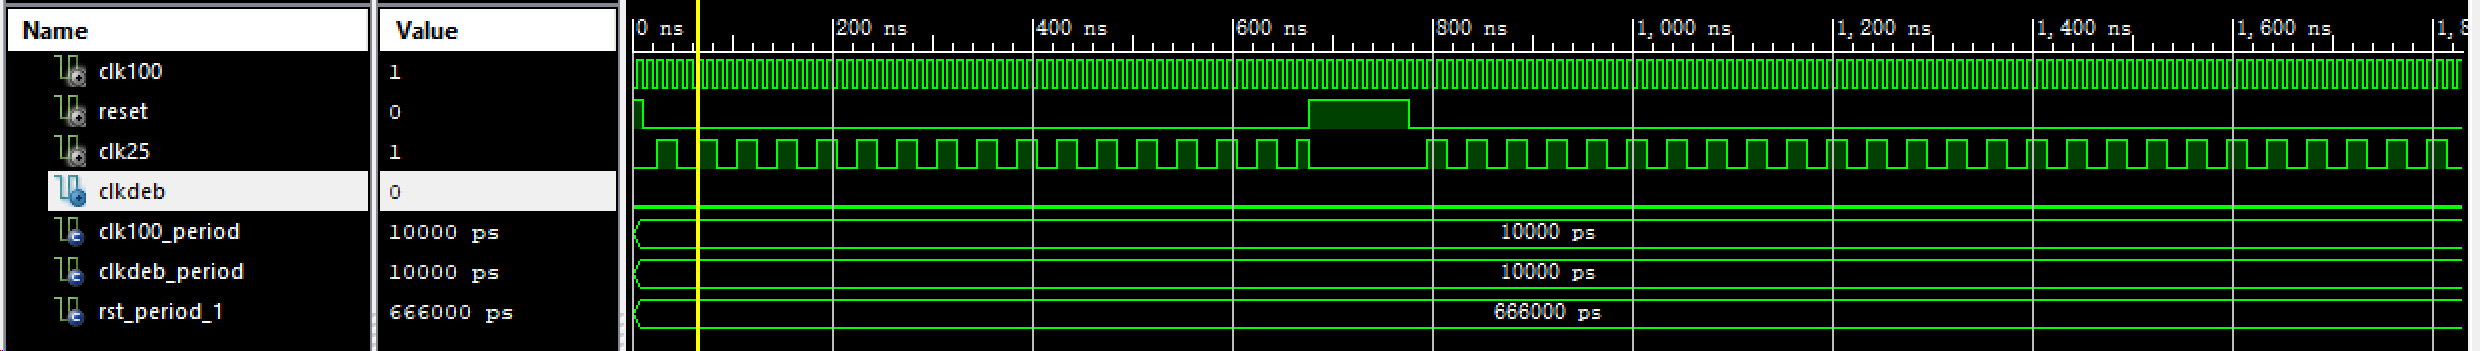
\includegraphics[width=1\linewidth]{homework3-2}
      \caption{The Simulation of Clock Unit (2)}
      \label{fig:homework3-2}
    \end{figure}
    \begin{figure}[h]
      \centering
      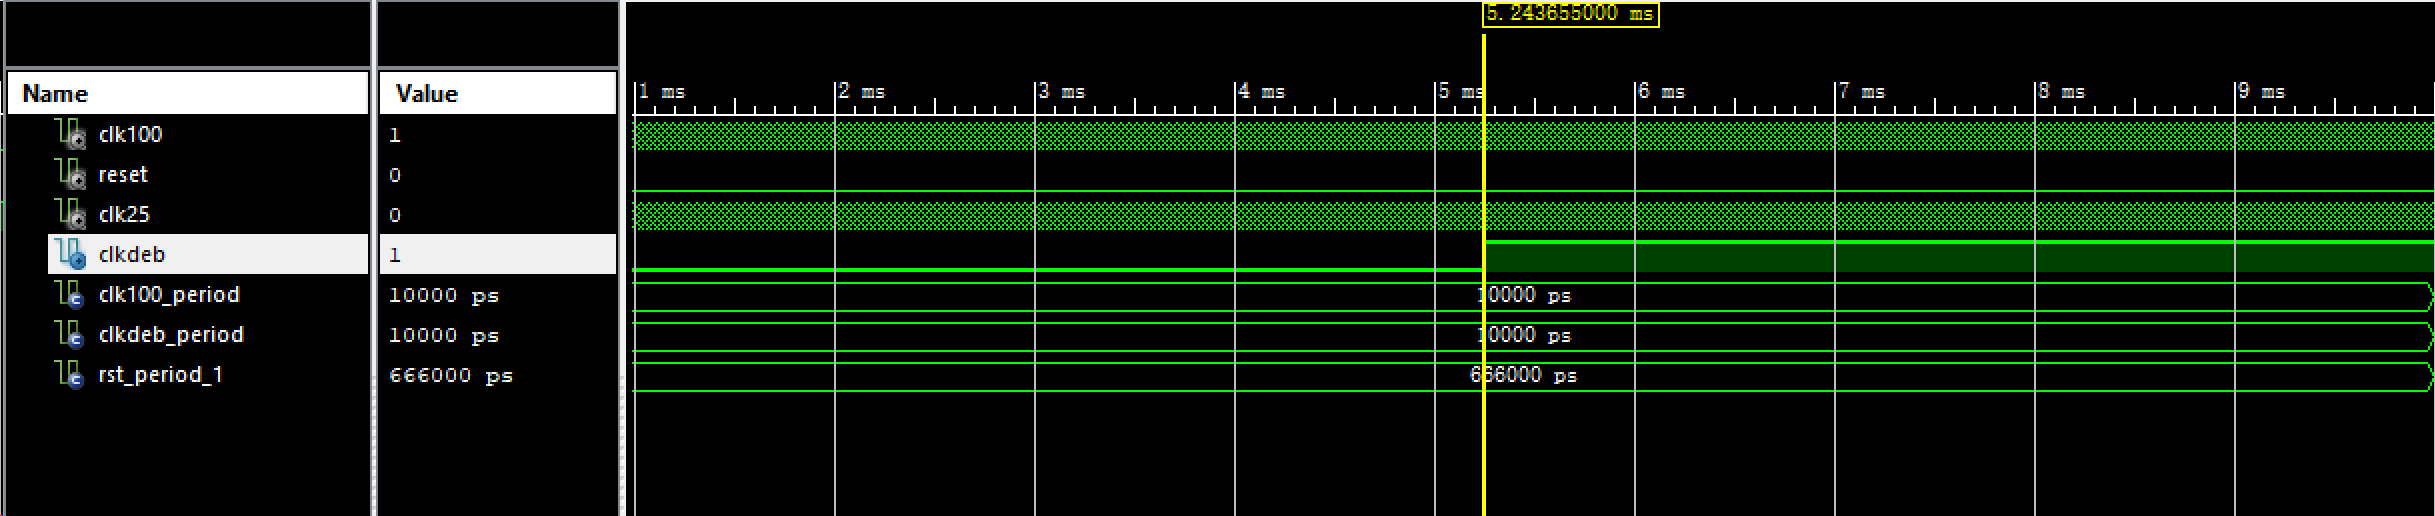
\includegraphics[width=1\linewidth]{homework3-3}
      \caption{The Simulation of Clock Unit (3)}
      \label{fig:homework3-3}
    \end{figure}

    \subsection{VGA Unit}
    \label{sec:ps:vgaunit}

    There are two main input for this unit: clock and item. The clock is for VGA to sync, 
    and item is to control what will be displayed.
    So we input a 100MHz clock for VGA, and because it is just simulation. And then we will input a signal for \verb|board_out|,
    to display what a pixel, or say block, or box, is.

    Just setting the clock signal turn over every 5 ns, and the signal of the \verb|board_out| will change in the range of
    ``border'', ``space'', ``food'', and ``snake's tail''.The it will display what is going on.

    And the final test bench file is like:
\begin{lstlisting}[language=VHDL,caption=VGA Unit Test Bench]
LIBRARY ieee;
USE ieee.std_logic_1164.ALL;
use work.game_package.all;

ENTITY tb_vga IS
END tb_vga;
 
ARCHITECTURE behavior OF tb_vga IS 
    COMPONENT vga
    PORT(
         reset : IN  std_logic;
         vga_clk : IN  std_logic;
         board_out : IN  cell_type;
         vsync : OUT  std_logic;
         hsync : OUT  std_logic;
         red : OUT  std_logic_vector(2 downto 0);
         green : OUT  std_logic_vector(2 downto 0);
         blue : OUT  std_logic_vector(1 downto 0);
         hor : OUT  integer range 0 to 799;
         ver : OUT  integer range 0 to 520
        );
    END COMPONENT;
    
   signal reset : std_logic := '0';
   signal vga_clk : std_logic := '0';
   signal board_out : cell_type := space;

   signal vsync : std_logic;
   signal hsync : std_logic;
   signal red : std_logic_vector(2 downto 0);
   signal green : std_logic_vector(2 downto 0);
   signal blue : std_logic_vector(1 downto 0);
   signal hor : integer range 0 to 799;
   signal ver : integer range 0 to 520;

   constant vga_clk_period : time := 10 ns;
	constant board_period   : time := 10 ns;
 
BEGIN
   uut: vga PORT MAP (
          reset => reset,
          vga_clk => vga_clk,
          board_out => board_out,
          vsync => vsync,
          hsync => hsync,
          red => red,
          green => green,
          blue => blue,
          hor => hor,
          ver => ver
        );

   vga_clk_process :process
   begin
		vga_clk <= '0';
		wait for vga_clk_period/2;
		vga_clk <= '1';
		wait for vga_clk_period/2;
   end process;
 
   board_process : process
   begin
	board_out <= space;
	wait for board_period;
	board_out <= border;
	wait for board_period;
	board_out <= food;
	wait for board_period;
	board_out <= snake_tail;
	wait for board_period;
   end process;

   stim_proc: process
   begin		
	reset <= '1';
	wait for 10 ns;
	reset <= '0';
        wait for 100 ns;	
        wait for vga_clk_period*10;
        wait;
   end process;
END;
\end{lstlisting}

    Then we can check behavioral syntax and simulate. Then we will get the output like  figure \ref{fig:homework3-4},
    figure \ref{fig:homework3-5}, and  figure \ref{fig:homework3-6}.


    \begin{figure}[h]
      \centering
      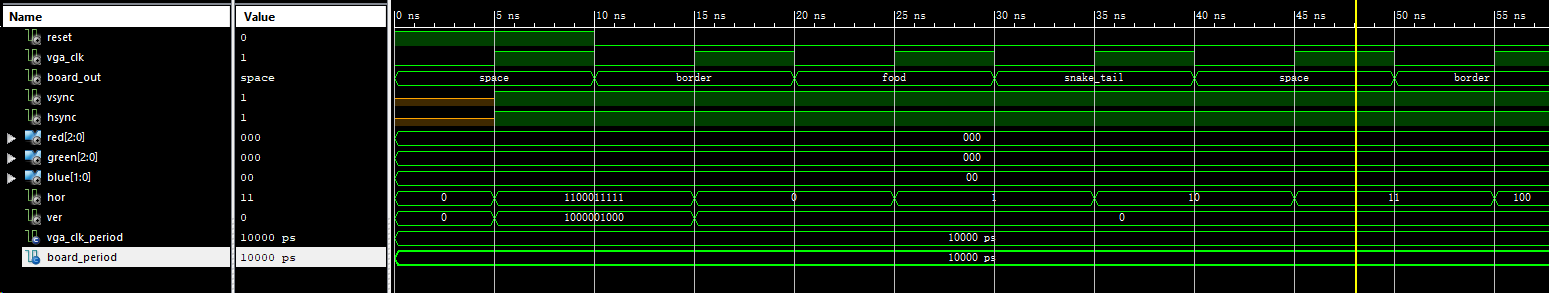
\includegraphics[width=1\linewidth]{homework3-4}
      \caption{VGA Unit Simlulation (1)}
      \label{fig:homework3-4}
    \end{figure}

    \begin{figure}[h]
      \centering
      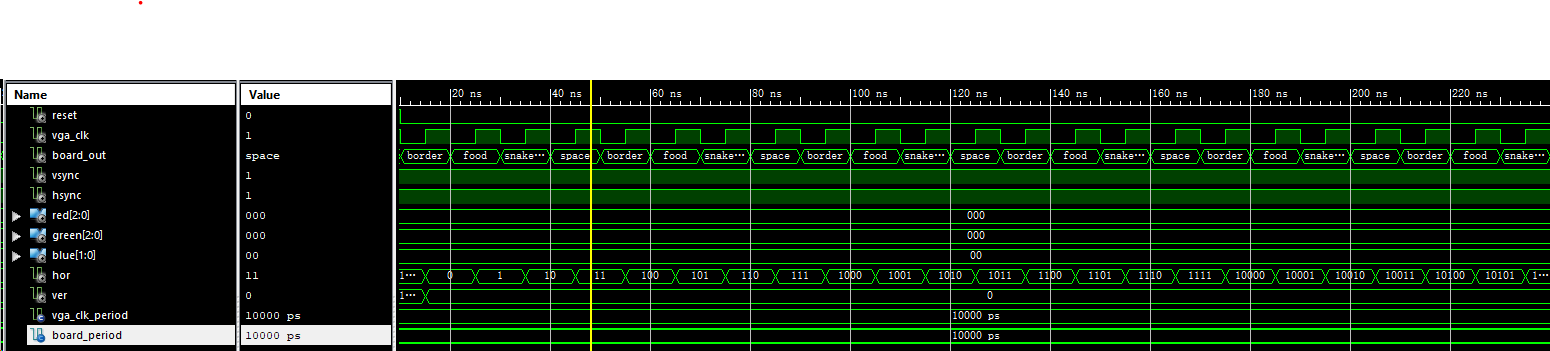
\includegraphics[width=1\linewidth]{homework3-5}
      \caption{VGA Unit Simulation (2)}
      \label{fig:homework3-5}
    \end{figure}


    \begin{figure}
      \centering
      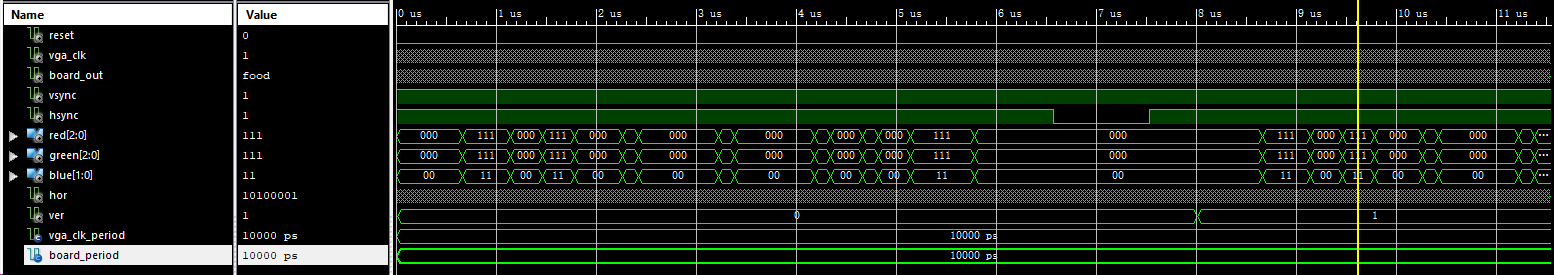
\includegraphics[width=1\linewidth]{homework3-6}
      \caption{VGA Unit Simulation (3)}
      \label{fig:homework3-6}
    \end{figure}


    \subsection{Game Logic Unit}
    \label{sec:gamelogicunit}

    
\end{document}